\section{Idea}
	The underlying idea of \textbf{RaceTrack} is a round-based racing game where players have to strategically choose their next move out of multiple reachable positions. These positions are calculated based on their previous turns and the position of other players. As the game calculates the selectable moves for each player based on their previous choices, the game gets more interesting and challenging with each passing turn. The players will be needed to demonstrate all their strategical and thoughtful decision-making skills to be able to beat their opponents. As the game is based on the original pencil and paper game \textit{Vector Race (also known as 'Racetrack' or 'PolyRace')}, the game can also help to improve the foresight thinking and basic understanding of vector mathematics of each player.

	\begin{figure}[H]
		\centering
		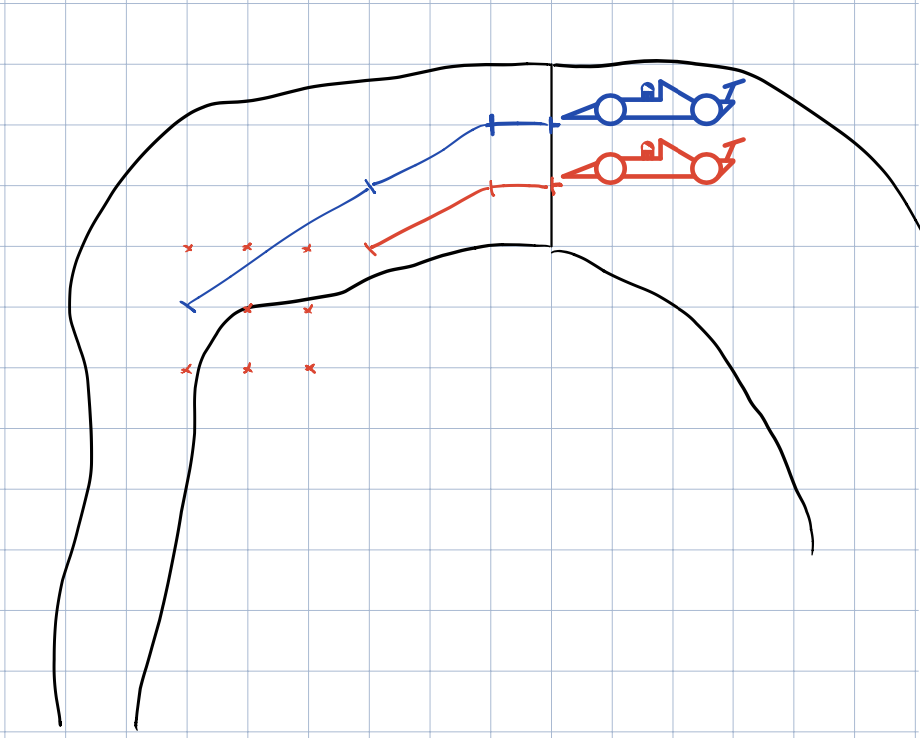
\includegraphics[width=14cm,keepaspectratio,center]{img/RaceTrack_Draft.png}
		\caption{Turn in the game (Mock-up)}
	\end{figure}